
\section{Abstract}
\label{sec:org3ea498f}
Analysis workflows which are based on the Fourier theorem are abundant in physics and engineering, yet rarely found in the biological literature.
They would be particularly useful in the analysis of locomotor kinematics, where movements can usually be broken down into repetitive cycles.
We herein repeat the basics of Fourier analysis and transformation to the frequency domain by reviewing previous studies which applied it in some form in the field of locomotor biomechanics.
We then discuss terminological and methodological heterogeneity among these studies, and point out some relevant properies of the method which have received relatively little attention.
One of the under-appreciated capabilities is that the transformation enables a diversity of multivariate analysis and modeling methods.
We demonstrate this by applying Fourier Series Decomposition, multivariate analysis and probabilistic modeling to a previously analyzed data set of bipedal walking kinematics in baboons.
The results are complementary to the prior analysis, and we find the capability to predict actual kinematic data for unobserved character combinations of particular interest for future kinematics research.


\FloatBarrier\clearpage
\section{Introduction}
\label{intro}

\subsection{Recurring Solutions}
\label{sec:org10ede19}
In 1822, a French mathematician initiated the remarkable discovery that any continuous signal, no matter how complex, can be represented by a sum of relatively simple trigonometric functions \citep{Fourier1822}.
Despite some initial limitations which were mended by scientists to follow, Fourier's work opened the door to the frequency domain.
Fourier analysis has become a widely-used tool in physics and engineering, whereas biologists have only occasionally made the transformation.
In particular, although it has been argued that the study of highly repetitive locomotor kinematics would benefit from applying Fourier methods \citep{Schneider1983,Pike2002,Skejo2021,Webb2007,Mielke2019}, it seems that few researchers have applied this simple method to date.
One reason for the hesitant adoption of the method are certainly terminological complexities in Fourier Theory.
These become apparent when assembling an overview of past attempts to apply related methods to locomotor kinematics.


In this study, we review the history of the application of Fourier Series in terrestrial vertebrate locomotion.

Some properties and practical misunderstandings are highlighted, before applying the method to a previously analyzed data set on bipedal locomotion in baboons \citep{Druelle2021} to once more demonnstrate the enormous potential of Fourier analysis.

This article is not targeted at a mathematically rigorous audience, who will certainly find shortcomings in the simplified explanations we provide.
Instead, we aim at facilitating the entry to the topic for applied biologists, especially in biomechanics.
Fourier Theory is well studied and widely applied, and numerous textbooks exist for all levels and fields \citep[\textit{cf.}][]{Bracewell2000,Osgood2019}.
The rich spectrum of Fourier-based methods comprises versatile techniques which would certainly facilitate the work on many relevant research questions in biomechanics.


\subsection{Fourier Series}
\label{sec:org276a6b8}

\begin{figure}[pt]
\centering
\includegraphics[width=.9\linewidth]{./figures/f1_jointangle.pdf}
\caption{\label{fig:jointangle}\textbf{Kinematic data generation workflow.} (A) Videos of animals are taken, here a baboon walking bipedally from left to right. The frames captured at touch-down, mid-stance, lift-off, mid-swing, and consecutive touch-down are shown. (B) Points of interests, e.g. joints, are digitized, which yields their pixel position over time. In this case the knee \(x\) and \(y\) positions are shown relative to their first value. Vertical bars indicate timing of the frames from the upper panel. (C) Joint angles are calculated from groups of three of those points of interest. Their change over time is a joint angle profile. We herein define joint angles to be zero at a fully extended (straight) joint, and positive for joint flexion. Per definition of ``steady state locomotion'', joint angles in steady state movement will return to approximately their start value over a cycle (indicated by the horizontal line, discussed below). Mathematically, this is called ``periodicity'', the joint angle profiles in steady state locomotion are thus ``cyclic''.}
\end{figure}

Typical kinematic measurements are joint angles, such as a hip angle, over time (but note that the following will equally apply to any continuous, periodic signal).
One recurrent unit of terrestrial locomotor behavior is a ``stride'', and it can go as follows (Fig. \ref{fig:jointangle} A).
If an animal walks, the distal part of its limb would touch the ground at a position ahead of the center of the limb.
Our example joint of interest, the hip, would then usually be highly flexed.
During stance phase, i.e. while the limb is in contact with the ground, the hip gradually extends, maybe reaching the lowest angle around the initiation of the swing phase.
While the limb swings forward to reach another touchdown, the hip joint flexes again.
Because the limb is a system of rigid bodies with a given mass, accelerations would never be abrupt, and the hip angle plotted over time might be described as a ``smooth sawtooth curve'', or even resemble a sine wave (Fig. \ref{fig:jointangle} C).
The change of a joint angle over time is called a ``joint angle profile''.


\begin{figure}[pb]
\centering
\includegraphics[width=.9\linewidth]{./figures/f2_domains.pdf}
\caption{\label{fig:domains}\textbf{The Frequency Domain.} Hip joint angle profile of bipedal locomotion in baboons. A visual representation (upper panels) contains exactly the same information as a numeric representation (tables / lower panels). Similarly, the information contained in frequency domain representation (right panels) is identical to that in the time domain (left panels). With the methods described below, one can transform from the time- to the frequency domain representation or back without loss of information. The frequency domain, which is accessible through Fourier Analysis formulas, is just a different representation of the data, and the transformation procedure is analogous to ``plotting'' (i.e. deterministic, reversible, favorable in some circumstances).}
\end{figure}


One could quantitatively capture joint angle profiles in different ways (Fig. \ref{fig:domains}).
The most intuitive, and by far most prevalent way is the time domain representation (Fig. \ref{fig:domains}, left column).
It stems directly from the technical method by which kinematic data is usually extracted: videos of the walking animals are digitized frame-by-frame \citep[\textit{cf.}][]{MMielke2020}.
The outcome are two columns of numbers: a ``time'', capturing the seconds at which a frame was captured, and then the ``angle'' measurement itself, usually assessed from three landmark positions (Fig. \ref{fig:domains}, lower left)
The more temporal sampling points, the better the temporal resolution, but the higher the digitization workload and storage requirement.


One assumption above is that the stride was recurrent, or cyclical, i.e. periodic.
This means that an almost (but not perfectly) identical stride will precede and follow the one of interest.
This is also called the ``steady state assumption'', i.e. the requirement that the observed behavior is regular (and thereby comparable to other observations).
Iff that assumption is met, the joint angle profile will start and end at approximately the same value, i.e. the hip angle at each limb touchdown will be almost the same.
Plotting this as angle against time will show a line with ends fixed on the left and right y-axes.
This is metaphorically the same situation as in a guitar string, which is fixed at both ends and performs some excursions from the zero line at positions in between.
To further stress this analogy, the hip joint angle profile can be described as the combination of a ``base tone'' and a number of ``harmonics'' (or ``overtones'').
Knowing the base and the relative contribution of the harmonics is sufficient to reproduce the ``sound'', or in other words to fully know the exact position of each element of the string or signal.
This is called the \textbf{``frequency domain''}, i.e. the representation of a cyclical signal by the relative contribution of its harmonics (Fig. \ref{fig:domains}, right column).
Any periodic, continuous signal, and thus also any cyclical joint angle profile, can be described like this, just as any tone the guitar string makes can be described as a sum of harmonics.
It might theoretically take infinitely many harmonics to exactly represent the signal (e.g. in case of non-smooth signals).
However, in practice, the effects which would cause this are usually considered to be measurement noise.
Physiological, ``real'' signals normally require few harmonics to be appropriately captured (discussed below).



How can Fourier Series be applied?
The method is based on the following formula \citep{Fourier1822,Gray1995,Bracewell2000,Mielke2019}, which is presented here for completeness and should not worry the reader.
\begin{equation}\label{eqn:fourier_coefficients}
c_{n} = \frac{1}{T}\sum\limits_{t=0}^{T} e^{-2\pi i n \frac{t}{T}} \cdot f(t)  \quad\quad \forall n>0
\end{equation}
Where \(c_{n}\) is a complex Fourier coefficient, \(T\) is the period of the signal or in our case the stride cycle duration, \(t\) is the time (i.e. ``x'' of the signal), \(f(t)\) is the signal (i.e. ``y'' of the signal), \(e\) is the Euler number, \(i\) is the square root of minus one.
The capital sigma tells mathematicians that this is a series, and thus the equation defines the \textbf{Fourier Series}.


At first, the analytical formula might seem quite complex for everyday application, and computer code might be more usable.
In appendix \ref{appendix:code} and in the supplements, we provide code for Python, R and Matlab which can just be copied and used\footnote{The "order" parameter in the decomposition is the number of coefficients to retain, which will be discussed in detail below.}:
\begin{lstlisting}{python}
coefficients = FourierSeriesDecomposition(time, signal, order)
\end{lstlisting}

It can be inverted (just as the analytical formula, see below):
\begin{lstlisting}{python}
signal = FourierSeriesRecomposition(coefficients, time)
\end{lstlisting}

Knowing the assumptions and limitations (see below) and paying attention to the data types and formats, these functions can be simply applied to transform between the time- and frequency domain.


\bigskip
There are numerous morphotypes of the Fourier theorem, which justifies a brief overview.
Equation \eqref{eqn:fourier_coefficients} is the exponential form of the Fourier Series.
The formula exists in other variants (which are equivalent by Euler's formula): the rare but useful ``amplitude-phase'' form, and maybe most notably the more abundant ``sine-cosine'' representation.
Historically, trigonometric functions are more convenient to handle, whereas modern computer implementations easily capture complex numbers, whereas humans have most intuition for amplitude and phase.
The Fourier Series is related to, but slightly different from, Fourier Transform, a relation which will be discussed in detail below (Ch. \ref{properties:transform}).
Applying the Fourier Series is a decomposition of a signal into its harmonic components, hence we will use the term \textbf{Fourier Series Decomposition (FSD)} herein.
``Discrete Fourier Transform'' (DFT) can be considered synonymous to ``Fourier Transform'', emphasizing the ``discrete'' nature of sampled data; ``Fast Fourier Transform'' (FFT) is an efficient algorithm to implement Fourier Transform.
DFT/FFT work on any signal and typically involve windowing, whereas FSD demands a periodic input signal.
FSD returns a single row of numbers (\textbf{``spectrum''}, i.e. harmonic contributions) for that signal, and that spectrum is discrete.
FFT natively also returns a spectrum \citep{Welch1967}, but a continuous one.
However, in practice, Fourier Transform is often applied in shifted windows and returns a ``spectrogram'' (i.e. frequency content over time).
Finally, a Fourier Series can be applied to a single angle (``1D''), or to multiple signals at the same time (e.g. on phase plots).
All of these (and other) variants of the method have been applied in the research of locomotor kinematics.

It is therefore worthwile to review the historic use of related methods in studies on locomotor kinematics, and look for some common patterns and strategies.

\FloatBarrier\clearpage
\section{Fourier Series in Locomotor Research}
\label{history}
The analogy of limbs and a pendulum was established early on \citep{Weber1836,Braune1895}, and maybe that is why Fourier Series was immediately among the relevant considerations for analysis.
To our knowledge, the first formal application of it was by Nikolas A. Bernstein \citep{Bernstein1927a,Bernstein1935}, who in the early years of his work was concerned with methodological advances in measuring motor actions \citep{Bongaardt2000}.
Bernstein suggested and applied a trigonometrical sum, which consisted only of sines and bares some resemblance in form to a Taylor approximation.

In his later work, Bernstein advocated a hierarchical organization of motor control \citep[\textit{cf.}][]{Bongaardt2000}.
This topic was taken up by studies in the field of motor learning, which would find evidence of higher order harmonics being affected by locomotor learning \citep{Gallistel1982,Marteniuk1983}.
Their methodology is overeall similar to that of Bernstein, yet improved by heuristics and standardization \citep{Jackson1979,Porges1980}.
The use of Fourier methods for asserting gait symmetry and variability were recognized \citep{Soudan1982}.


Van Weeren \emph{et al.} applied Fourier Series to measure skin marker displacement, not joint angles \citep{vanWeeren1992}, yet extracted the coefficients with a regression instead of direct transformation (see below).
Schendel and colleagues quantified inter-vertebral angles with a sine-cosine Fourier Series \citep{Schendel1995}, again with a computational regression.
It was found that relatively few harmonics can be sufficient to detect symmetry and lameness in horses \citep{Audigie1999,Peham1996}.
Others have applied a Fourier Series to the segment angles of limb segments \citep{Grasso2000}, for example to infer amplitude and phase relations.
Fourier Series has recently been applied to the specific analysis of human running \citep{Skejo2021}.


Two studies stand out from the previously mentioned, conventional uses of Fourier Series.
\citet{Pike2002} have made use of the data transformation to perform multivariate, quantitative comparison of kinematics across a broad range of taxa.
Their focus lies not on the method itself and the generated coefficients, but rather on downstream data processing methods.
Another hallmark study in terms of advocating Fourier Series in locomotor research is that of \citet{Webb2007}.
The authors provide a comprehensive introduction to the method, list its advantages and fields of application as well as future perspectives.
Thereby, the article has outstanding educational value for those attempting to find a start with the method.


With the rise of computational approaches, inverse dynamic modelling of human gait was facilitated by transforming to the frequency domain \citep{Ren2007}; pattern recognition and classification methods were applied \citep[e.g.][]{Mostayed2008}.
Along these lines, Fourier Series was used to get a frequency spectrum and compute development- and pathology related change in overall locomotor frequency \citep[e.g.][]{Kurz2011}.
Multi-Dimensional variants of Fourier analysis for two angles in phase plots or ``cyclograms'' \citep{DiBerardinoIII2010} or for 3D angles using Quaternions \citep{Kenwright2015} point at promising future directions.


Finally, recent work by the authors has expanded on the aspect of multi-variate analysis and favorable data properties in the frequency domain \citep{Mielke2019,Mielke2023}.


Overall, although some references exist, the studies using Fourier Analysis are sparse among locomotion literature.
Authors who apply the technique tend to emphasize its usefulness, but often seem to be unaware of previous implementations.
Few studies have explored downstream analysis of the Fourier coefficients.
Confusions about mathematical terminology (e.g. ``series'' or ``transform'', ``transformation'' or ``regression) complicate the situation.
To summarize, variability in the use of Fourier Series arises from the following questions:
\begin{itemize}
\item Which signals to use? (joint/segment angles)
\item How to apply the transformation? (no regression required, see below)
\item Which form and implementation to use? (``Series'' vs. ``transform'', ``trigonometric'' versus ``complex exponential'' form)
\item If and how to process data in the frequency domain? (multivariate analysis, modeling)
\item How many coefficients to retain? (order)
\item The possibility of inverting FSD has been neglected, maybe in consequence of the above.
\end{itemize}

All these questions are the purpose of this review, and will be adressed below.

\FloatBarrier\clearpage
\section{Properties of the Fourier Series}
\label{properties}
A lot of the text below is written from the applied perspective of a biologist, who used the transformation and its inverse to actual data.
Not all of the reported properties of Fourier methods are directly linked to literature references, but most general courses and textbooks cover these concepts \citep[e.g.][]{Bracewell2000,Osgood2007,Osgood2019}.


\subsection{Not a Regression}
\label{sec:orged49846}
As pointed out above, some researchers have applied regression algorithms to extract the weights of the harmonics contributing to the signal of interest.
A regression is an iterative procedure which attempts to match a known, parametrized function (the model) to a target signal (the measurement) by adjusting the parameters with clever adjustment rules.
An intuitive example is linear regression, in which the parameters `a` and `b` of a function \(y=a+b\cdot x\) are adjusted so that the formula best describes the observed data relation of `y` and `x`.
Typical optimization algorithms are the Nelder-Mead simplex \citep{Nelder1965} or variants of the BFGS algorithm \citep{Broyden1970,Fletcher1970,Goldfrab1970,Shanno1970,Zhu1997}.
Though it is immensely useful, regression has several technical disadvantages: convergence is not guaranteed, start values are required and might affect the result, the algorithm might get stuck in local optima, accuracy is finite, the iterative procedure is computationally expensive, and reversibility requires the inverse function and another regression.
Some of these disadvantages are emphasized when working with trigonometric functions.


\textbf{Fourier Series Decomposition is not a regression.}
Determining the ``parameters'', i.e. Fourier coefficients, works by eqn. \eqref{eqn:fourier_coefficients}, which can be directly translated to computer code (see above and appendix \ref{appendix:code}).
The procedure is deterministic, exact, and reversible; no start values are required.
The trigonometric formulas provided in many publications resemble regression models, but applying a regression procedure is not necessary.
We will demonstrate the overall procedure below and provide code for some relevant scientific scripting languages as proof of concept.


\subsection{Relation to Fourier Transform}
\label{properties:transform}
As discussed above, Fourier Series Decomposition (FSD) requires a signal of finite length which starts and ends at the same value (periodicity).
It computes a discrete spectrum of the whole function, i.e. the amplitudes for each harmonic.
A generalization of FSD is the Fourier Transform, which does not assume periodicity, and which can be applied to signals of indefinite length by shifting a computation window along the signal.
Fourier Transform yields continuous spectra, measuring frequency content in units related to absolute time.
When applied in a sliding window, Fourier Transform provides a spectrogram of the signal, i.e. the changing contribution of different frequency components to the signal over time.
The minimum frequency is limited by the window width, the maximum frequency is determined by the sampling rate of the signal \citep{Shannon1949}.
Fast Fourier Transform (FFT) is the most common algorithm for computation \citep[\textit{cf.}][]{Heideman1984}, and FFT is readily available in most programming environments.
Note that there are many other such transforms which circumvent some limitations of FFT or might be otherwise useful in research, such as the S-Transform \citep{Stockwell1996,Brown2010} or Empirical Mode Decomposition with the Hilbert-Huang Transform \citep{Huang1998}.


The result of FFT on a single window is a quasi-continuous frequency spectrum, and the frequencies are related to absolute time.
Because of this, joint angle profiles which look exactly identical, but differ in stride duration, would have different frequency spectra.
In contrast, FSD only considers harmonics, which are the integer multiples of the signal period.
Therefore, the outcome of FSD is usually a much shorter array of numbers (Fourier coefficients).
The FSD formula involves a normalization for the signal period (i.e. stride cycle duration), and thus strides of different duration can be directly compared (but see below).
FSD also avoids problems of FFT which are due to windowing.
Though both procedures could be applied to stride cycle kinematics, \textbf{FSD is favorable if the periodicity/cyclicity assumption holds}.


\subsection{Time Scale Independence}
\label{sec:org18025b1}
Another favorable property follows from the cyclicity: \textbf{Fourier coefficients are independent of temporal scale or sampling}.
Due to the normalization mentioned above, the FSD of the signal does not contain any information about the original duration of the signal (e.g. stride duration), nor does it matter much where the cycle started.
On the inverse FSD, a new time frame and temporal sampling must be chosen.
It is thus possible to re-sample the time line of a measurement by transforming it to the frequency domain, and then back with a different timeline.


In consequence, FSD is useful for homogenizing and comparing signals of variable duration.
This can be advantageous, if groups or paradigms of variable stride durations are to be compared.
If discarding that information is unintended, ``duration'' can simply be retained as a separate variable.
The same holds for speed and other collective variables which are related to the temporal structure of the signal.

It follows that \textbf{Fourier coefficients do not replace collective variables (e.g. duration, speed), but complement them}.
In case of joint angle profiles, Fourier coefficients capture the kinematics, while collective variables quantify the system outcome as a whole.
Both are related by morphology (i.e. limb segment dimensions), which is another relevant class of variables that can and should be associated with kinematics in modeling approaches.


\subsection{Approximate Periodicity}
\label{properties:endstart}
How ``flexible'' is the periodicity assumption?
Motor behavior underlies variability \citep{Bernstein1935}, thus one might never measure a perfect end-start match.
Fourier Series Decomposition works on noisy signals, yet it should be assured (as a technical requirement) that the end-start-difference is smaller than the white noise.
There are a few common strategies to accomplish this if it is not given, and it has to be discussed how these strategies affect the outcome.



Firstly, one could ignore a start-end-difference, and bluntly apply FSD.
The algorithm assumes periodicity, but the formula has no means to check this assumption, and will hence ``connect'' the last and first sample.
This would lead to an abrupt change, which demands high order harmonics, which will show in the spectrum.
However, abrubt changes from discontinuities are not physiological, so those values can be considered an artifact.


As a second option, it is common practice to generate an inverted version of the signal (of the form \(g(t) = -f(-t)\) ) and concatenate it to the end of the original signal.
This could be visualized as a rotation of the signal about its last measurement point, which results in the values progressing first in forward and then inverted in backward measurement order, all changes cumulating to zero, and the signal ending where it started.
This method is common in the Fourier analysis of ground reaction force measurements \citep{Schneider1983,Alexander1980}, where data usually starts and ends at zero.
It nihilates the signal mean (zero'th component) and shifts all consecutive harmonics up by one due to period doubling.
The rationale of using this method is that it generates symmetry and smoothness, which generally reduces the order (i.e. number of harmonics) required to retain all relevant infromation of the signal.


A third method to mend end-start differences is to simply spread them over the whole period of the signal \citep{Mielke2019}.
This can be achieved in a computationally efficient way by subtracting an array of numbers from the signal which is linearly increasing from zero to the end-start difference, and which has the same number of samples as the signal (pseudo-algorithm: \texttt{signal -= linspace(0, end-start, number\_of\_samples)}).
For this to be valid, it must be ensured that the end-start-difference is negligible in magnitude, non-physiological, and non-systematic.
If those are givens, spreading the difference over the cycle is least invasive with regard to the outcome coefficients.
As with the previous method, this smoothes the signal and reduces higher order components, yet without the caveat of altering the relation of relevant harmonics.



\begin{figure}[pt]
\centering
\includegraphics[width=.9\linewidth]{./figures/f3_endstart_Procrustes.pdf}
\caption{\label{fig:endstart}\textbf{Stride cycle end-start matching.} A stride cycle can be defined as the time interval between two frames which have the highest similarity in joint configuration and enclose exactly one swing and stance phase. (A) Putative start and end frame configurations, superimposed onto the original video frames. Several frames are candidates for cycle end, indicated by the series of cross markers. (B) Superimposition of end frame candidates onto the reference start frame, using Procrustes Superimposition. Only the axial line points (head to toe) are used for superimposition. (C) Configuration difference (measured as Procrustes distance \(pd\), shifted by the arbitrary formula \(log\left(pd*10^3+2\right)\) for visualization) over the whole stride cycle for different candidate start frames. (D) A heatmap of configuration difference can identify mathematically optimal stride cycle intervals. Dashed black crosshair: cycle start and end, conventionally determined by limb touch down. Blue crosshair: start and end frame with maximal configuration similarity, i.e. minimal Procrusted distance of the configurations at candidate frames.}
\end{figure}

If used with caution, the third method is the favorable one for applications on locomotor kinematics.
However, with that sort of data, there is another relevant method to minimize end-start-differences.
The \textbf{choice of where the start and end of a cycle lie} is conventionally made by finding the (left hind-limb) touchdown.
This time point is more or less distinctly visible on videos, and might be a requirement for data comparison.
Yet, mathematically, that is just an arbitrary point in the cycle, and biomechanically, the configuration of the limb can be different on two touch downs (two strides might instead have higher cross-resemblance just before touchdown, or at mid-stance; Fig. \ref{fig:endstart}).
The term configuration herein describes the relative spatial arrangement of a set of points of interest or markers.
Thus, if emphasis of the analysis lies more on the cyclic character of the stride, and if researchers find it valid to choose a different point for start and end of the cycle, then optimal points could be found automatically by cross-comparing the configurations of the whole limb in a sufficient frame range around the limb touch downs \citep[as applied in][]{Mielke2019,Mielke2022}.
This can be achieved by taking all relevant points digitized in the videos (treating them in each frame as a geometric shape; Fig. \ref{fig:endstart}B) and calculating the Procrustes Distance between those frames or shapes \citep{Rohlf1990}.
That Procrustes Distance is a direct measure for the configuration difference between frames (Fig. \ref{fig:endstart}C).
In a cross-comparison, the two frames which have least Procrustes Distance are candidates for start and end of the cycle (Fig. \ref{fig:endstart}D), and should be verified by visually superimposing the video frames.
Conversely, whether or not there are two such frames with a sub-threshold Procrustes Distance, and at what time in the cycle they appear, can be a useful proxy to confirm steady-state locomotion.


All these are technical tricks which usually improve the data set quality and consistency.
The bottom line is that, in steady state locomotion, the \textbf{periodicity assumption is usually met}, and there exist minimally invasive adjustments to ensure that the data strictly meets the mathematical requirements of FSD.



\subsection{Reversibility}
\label{sec:orgfb5d796}
Some data operations can be undone (math.: invertible, i.e. reversible), others not.
For example, consider the Euclidean vector norm of a temporal series of velocity vector measurements: the resulting number (speed) can quantify the magnitude of the original velocity vector, but not its direction.
Conversely, when modeling speeds depending on some other parameter and predicting magnitudes, or when averaging speeds, one could not infer a direction.
Information is lost in the transfromation from a three-dimensional vector to a single number representing its length.

Other operations are invertible: consider again a series of velocity vectors of a physical object moving in space.
One can freely change the reference coordinate system.
Moving from an earth-bound reference frame to the coordinates defined by the object and back is possible without loss of information.
Another common, invertible coordinate transformation is the Principal Component Analysis, which transforms data into the space spanned by the orthogonal eigenvectors of a data covariance matrix.
Because these transformations retain all information, and because an inverse mathematical operation exists, one can move the given data forth and back between the different spaces or domains.
Even more, one can transform or untransform unrelated, new data between spaces, although that data was not involved in calculating those spaces.
This feature is useful and common for averages and extrapolations.


Fourier Series Decomposition is invertible.
As described above, it translates the data from a ``time-dependent array'' form to a time-independent, complex-valued frequency space.
Any set of values, be they observed or synthetic, can also be translated back via an inverse operation.
In contrast to PCA, this does not even require the eigenvectors of the original data (there is only one frequency domain).
Some operations, such as averaging of multiple signals, are equivalent in the time- and frequency domain.

The formula for the inverse Fourier Series is the following:
\begin{equation}\label{eqn:fourier_inversion}
	f(t) = \sum\limits_{n=0}^{N} (2\cdot c_{n})\cdot e^{2\pi i n \frac{t}{T}}
\end{equation}

Notation herein as in \eqref{eqn:fourier_coefficients}, with \(N\) being the order (number of coefficients).
Computer code for application in R, Matlab and Python can be found in appendix \ref{appendix:code} and the supplements.

The existence of this inverse formula means that just as exchanging a coordinate basis for linear coordinates, \textbf{one can convert freely between time- and frequency domain}.


However, one limiting factor is the order of the Fourier Series.
Some signals (i.e. those with sharp turns or quick changes) require a high number of harmonics to be accurately represented in frequency space.
Conversely, when operating with a finite order, some signals might be filtered on the first transformation to the (pruned) frequency domain.
Real measurements are usually subject to Gaussian noise, such noise involves changes as quick as measurement sampling, and thus it is lost in FSD.
This \textbf{filtering property of FSD} can represent a loss of information (if the noise is considered informative, but note that in that case the residual after re-transformation might be even more informative).

However, in cases where this filtering effect is negligible or even favorable, FSD and its inversion can be applied.
Repeated back- and forward transformation does not discard further information.
When implementing a version of the equations above in computer code, a good check is whether values are unchanged after applying FSD and its inversion in series.
And because of the relatively few coefficients needed for accurate representation of physical processes, compared to sampled timelines, it is often \textbf{efficient to store} kinematic data in the form of FSD coefficients.

\subsection{Choice of Order}
\label{sec:orgff5edd5}
How to decide how many coefficients should be retained?
That number is the ``order'' of the Fourier Series.
It can be easily determined by exploiting the reversibility of a method.
Each data point (i.e. each measured joint angle profile) should be converted to the frequency domain with a given order, and then converted back to the time domain.
The (root-mean-square) difference of the original signal and the re-transformed one should be small in magnitude and normally distributed around zero.
Additionally, original and re-transformed signals should be plotted on top of each other for visual inspection.


This strategy is of general use, and we will demonstrate it on the test case below (ch. \ref{casestudy:dataprep}).
In the particular case of joint angle kinematics, it has often been concluded that relatively few coefficients are sufficient to capture the essence of the phenomenon.
This is physically plausible, because the elements of limbs are rigid bodies with a certain inertia.
Such elements cannot perform too abrupt accelerations, and in consequence, the profiles are smooth.
Furthermore, in the case of steady-state locomotion, the ensemble of rigid body elements produces the behavior, and it is unlikely that any single element can oscillate an order of magnitude quicker than the whole limb.
The stride cycle is the defining time interval, and normally all elements move in relative unison, which limits amplitude in the higher order coefficients.


\subsection{Affine Components}
\label{sec:org05eb5a7}
Some attributes of a signal are emphasized by Fourier methods.
Those can be summarized intuitively as those attributes of the signal which can be changed without altering the ``perceived shape'' of the signal.

The most obvious one is the average of the signal over time, i.e. its \textbf{mean value}.
When changing the mean of a signal in the time domain by adding the same scalar value to every sample, the signal shifts ``up and down'', but retains its temporal structure.
The mean is completely captured by the zero'th coefficient, which therefore is always a real number.
Apart from that, changing the mean of a signal leaves its frequency domain representation unchanged.

Another attribute of the signal is the \textbf{amplitude}, or how much values change around the mean.
In the time domain, amplitude is altered by centering the signal and multiplying it with a scalar, followed by un-centering.
In the frequency domain, amplitude is visible as the distance of coefficients from the origin of the complex plane (i.e. the cumulative magnitude of the complex numbers, or the norm of the complex coefficient vector).

The third special signal aspect is \textbf{phase}, and it has to do with the periodicity of the signal.
Phase is quantized in the time domain by sampling, and it can be changed by taking a number of samples from the end of the signal and appending it to the start (``rolling'' the signal around, or changing the start point of the cycle).
In the frequency domain, changing the phase rotates the coefficients in the complex plane (but note that higher order coefficients rotate exactly \(n\) times quicker).
Because the frequency domain is independent of sampling, phase can be changed by any scalar number here, and is not limited to the sample raster.
This allows efficient temporal resampling, as wel as an optimal alignment of multiple signals \citep[\textit{cf.} supplementary information of][]{Mielke2019}.
Phase is an angle, best used in the range of zero and \(2\pi\).
It is changed in the frequency domain, just as any rotation in a complex plane, by multiplication of a complex exponential \citep["delay/shift theorem", \textit{cf.}][]{Bracewell2000}.

The fact that amplitude is the distance and phase the angle of Fourier coefficients in the complex valued frequency space illustrates the relation of the exponential and amplitude-phase form of the Fourier formula: the latter are just the corresponding polar coordinates.


Mean, amplitude and phase are called \textbf{affine components} of a signal, which describes the fact that they can be adjusted by scalar operations without altering the ``signal shape''.
They can even be standardized (mean: zero, amplitude: one, phase: zero).
They can be associated with biological meaning: the mean quantifies dynamic posture, the amplitude is related to effective range of motion, the phase quantifies relative timing of joint movements.
What remains after standardization, i.e. after isolation of the affine components, is in a way the essence of a signal, its ``shape'', which is defined by the temporal (or frequential) structure of the behavior.
In the case of joint angle profiles, this remainder can be considered coordination \emph{sensu strictu} \citep{Mielke2019,Mielke2022}.

\subsection{Multivariate Analysis}
\label{sec:org8b03db5}
The numeric representation in the frequency domain is usually shorter, and as mentioned above, storage might be efficient.
Nevertheless, an FSD of the order \(N\) will yield \(N+1\) coefficients, which are \(2N+1\) numbers when splitting up their real and imaginary parts.
Although we usually find an \(N<10\) appropriate (see above), this would still leave a considerable amount of variables for analysis.

This raises the question of the effect of multivariate analysis methods, such as Principal Component Analysis (PCA).
PCA is a coordinate transformation which finds orthogonal coordinate axes in the data set that are oriented towards the largest variability within the data.
A common purpose of PCA is dimensionality reduction, and it is particularly effective if there are strong co-variations within the data.
It seems clear that Fourier coefficients of a single joint angle profile are intrinsically linked, for example through the phase rotation in the complex plane (exponential form).
However, it is not obvious whether that holds any advantages for PCA, because the phase rotation does not cause linear correlation.
On the other hand, higher coefficients are usually of lower amplitude than the main coefficients, and thus their putatively relevant variability might be lost in a PCA-based dimensionality reduction.
Thus, PCA does not generally hold benefits for the analysis of single joint FSD in its complex exponential formulation.
It might be different in the apmlitude-phase formulation, which should be explored in future research.


If more than one joint is of interest, coefficient number is multiplied, but the situation for multivariate analysis changes.
Different joints are often interrelated through adjacency along their linking segments.
Biarticular muscles and tendons can cause correlated movements, which makes top-down sense, because a typical vertebrate limb during swing phase tends to be extended and flexed altogether.
This situation is favorable for PCA, in a sense that dimensionality reduction can often be achived with relatively little information loss.
Note, however, that PCA must be adjusted in a way that accounts for the FSD properties as follows.
It is common practice and often advisible to standardize input variables prior to PCA, so that their value ranges are comparable (usually done by subtraction of the mean and division of a variability measure).
Such a standardization would disrupt the temporal structure of the signal, and emphasize nuisance variability in higher order coefficients.
A better strategy for multi-joint analyses is the standardization by removal of affine FSD components.
As mentioned above, mean joint angle and joint amplitude can be standardized, and phase differences of all observations can be minimized by temporal alignment.
With such preprocessing, the outcome of a PCA will equally represent each joint of interest, without disrupting the temporal structure of the joint angle profiles, and benefitting from intrinsic correlations of movements of the limb elements.
PCA is invertible, and any downstream modeling outcomes can be related back to the original joint angle profiles.

\FloatBarrier\clearpage
\section{Case Study: Predicting Bipedal Walking in Adult Male Baboons}
\label{casestudy}
Above, we re-iterated some fundamental properties and best practices related to Fourier Analysis, and Fourier Series Decomposition in particular.
We will now outline the typical workflow of the analysis of kinematics with that method, focusing only on the steps which are affected by the Fourier method.
There is a lot of flexibility in the procedure (see Fig. \ref{fig:procedure} for a coarse guideline), and researchers should feel encouraged to adapt the steps to their needs.
For illustration, we apply the steps outlined below to a previously analyzed data set of bipedal walking in olive baboons, \emph{Papio anubis} \citep{Druelle2021}.

\begin{figure}[pt]
\centering
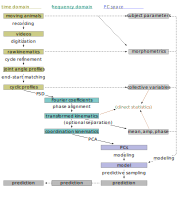
\includegraphics[width=.9\linewidth]{./figures/f8_flowchart.pdf}
\caption{\label{fig:procedure}\textbf{Analysis and Modeling Procedure.} Workflow overview of the preparation, transformation and analysis steps involved in the data analysis on baboon bipedal walking as described in the text, from raw observation (top) to statistical inference and multivariate analysis (bottom). At each point of the procedure, transformation between the domains is possible and quality checks should be performed.}
\end{figure}

\subsection{Data Preparation}
\label{casestudy:dataprep}
After data acquisition is complete and hard drives are filled with videos, the individual stride episodes which were captured on video must be annotated and extracted.
As a good approximation, one can use the conventional touch down timepoints (though lift off or mid stance would work equally well, and the choice may vary within the dataset).

\begin{figure}[pt]
\centering
\includegraphics[width=.9\linewidth]{./figures/f4_raw_inspection.pdf}
\caption{\label{fig:raw_inspection}\textbf{Raw Data Inspection.} (A) Plotting a series of stride cycles in the camera reference frame can aid the identification of data discontinuities (visible here in the distal limb markers). The animal is moving from left to right. A stick figure displayed for the last frame facilitates landmark attribution (torso, tail, hind- and forelimb are shown, similar to Fig. \ref{fig:endstart}). (B) Plotting one stride in the moving reference frame of the subject (zoomed in on the limbs) can confirm cyclic/steady state movement.}
\end{figure}


A prerequisite for any meaningful analysis is consistent, complete data.
Data in this case are points of interest, tracked on videos.
There are many tools for video digitization, which are more or less automatic and accurate \citep{MMielke2020,Knoerlein2016,Hedrick2008,Crall2015,Mathis2018,Karashchuk2021,Dunn2021}.
It should be assured that no frames have been involuntarily skipped in the process of tracking, and that there are no discontinuities in the series of point positions.
This can be easily achieved by plotting the time series of digitized points, either in the global reference frame, or in a moving reference associated with the subject (Fig. \ref{fig:raw_inspection}).
After digitization, the aforementioned calculation of Procrustes distances between putative start and end frames (ch. \ref{properties:endstart}) can be used to refine the stride interval and minimize end-start-differences.

With strides identified and data quality assured, collective variables such as duration, speed, clearance, or gait asymmetry can be stored for each stride observed in the dataset.


Next, joint angles can be calculated in a variety of ways.
Their precise definition and direction is arbitrary, yet should be consistent and clearly documented.
Care should be taken that joint angles do not show jumps at any time point of the movement, for example by crossing the \(2\pi\) angular interval border.
Such jumps would lead to a wrong FSD, because that procedure does not natively consider angular value ranges or interval wrapping and thus treats the jump as if it were an actual discontinuity.
The joint angle definition chosen herein, with fully extended limb corresponding to a joint angle of zero, and angles ranging from \(-\pi\) to \(+\pi\), usually avoids such discontinuities.

In the case of two-dimensional joint coordinates, calculation of joint angles is relatively straight forward with an `arctan` formula.
When working in three dimensions, the question is whether sufficient anatomical reference points can be digitized to calculate actual anatomical joint angles.
If not, it must be sufficient to calculate a single angle between the segment vectors, though that does not necessarily correspond to anatomical degrees of freedom.
If instead there are sufficient reference points, multiple rotation axes and angles per joint can be used and integrated just as in a multi-joint analysis (see below).
Note that there have been attempts to directly calculate Fourier coefficients from 3D joint angles, using quaternions \citep{Kenwright2015}, which would be the most elegant solution for this purpose.


After removing end-start-differences as described above (ch. \ref{properties:endstart}), joint angle profiles are plugged into the Fourier equation \eqref{eqn:fourier_coefficients}, e.g. by using the corresponding programming functions supplemented to this manuscript.
Thereby, joint angle profiles are transformed to the frequency domain.
Though we above emphasized the complex values of the coefficients, they can as well be represented by a one-dimensional array of alternating real- and imaginary parts of the coefficients.
The transformation should be inverted, and original and re-transformed joint angle profiles plotted together, to exclude coding errors and confirm that order was chosen high enough (Figs. \ref{fig:reversibility}, \ref{fig:residuals}).

\begin{figure}[pt]
\centering
\includegraphics[width=.9\linewidth]{./figures/f5_reversibility.pdf}
\caption{\label{fig:reversibility}\textbf{Reversibility.} A single joint angle profile, processed forth and back with Fourier Series Decomposition (green, using 9 coefficients) and Principal Component Analysis (orange, using first 5 principal components, after FSD). The residual \(\epsilon\) is the mean of Euclidean distances of all angle measurements over time from their corresponding re-transformation in the time domain. See also Fig. \ref{fig:residuals}.}
\end{figure}

\begin{figure}[pt]
\centering
\includegraphics[width=.9\linewidth]{./figures/f6_residuals.pdf}
\caption{\label{fig:residuals}\textbf{Retransformation Residuals,} (A) after performing FSD only with a given order (i.e. number of coefficients, x-axis), (B) after FSD (9 coefficients) and PCA with a given number of retained components. Residuals \(\epsilon\) (y-axis) as defined above. Joint angle profiles of all observed baboon strides are included, the distribution of residuals is indicated by grey ``violins''. Relatively low numbers of coefficients and components are sufficient to get close to the asymptotic accuracy. The absolute residual is joint-dependent (compare hip and knee, for example), an effect which is primarily determined by digitization accuracy and measurement noise. The data point for ``full'' PCA dimension is the reference value with just the FSD.}
\end{figure}

\subsection{Multivariate analysis}
\label{sec:org10a29bf}
Each stride processed in the analysis counts as exactly one data point, and so far, data points were considered independently.
The conventional next step is to analyze their relation to each other.

For example, it might be apparent that two or more data points are phase shifted relative to each other: all the characteristic maxima and minima of the joint angle profile would appear later or earlier in the time domain plot.
If we assumed that strides are cyclic, we must conclude that these phase shifts are due to our arbitrary choice of the start point within the cycle.
Phase differences should therefore be minimized.
However, different joints, when analyzed together, might theoretically give contradicting information on the relative phase shift of different strides.
Obvious solutions are to either choose a reference angle for phase alignment (this might be an angle not otherwise used for analysis: in the baboon test case, we chose the ``total limb'', i.e. the head-hip-toe angle), or to use an amplitude-weighted average phase shift as calculated from all joint angles of interest together.

And just as with phase, there are design choices about whether to keep the other affine components (mean, amplitude) implicit in the multivariate data set, or extract and isolate them for subsequent analysis.


Independent of these choices, the result of the previous steps is a data table consisting of multiple observations (strides, in rows) and variables (Fourier coefficients, in columns).
The observations can be related to their corresponding master data (i.e. subject characteristics, morphology, collective variables, isolated affine components) by a simple stride index.

Such a data structure is eligible for multidimensional analysis methods, and one of the simplest such method is Principal Component Analysis (PCA).
Often, PCA justifies a significant reduction of data dimensionality (i.e. number of data columns), depending on how much variance is concentrated on the first components.
Apart from the residual variance not covered by the retained principal components, PCA is again information preserving and reversible (which should be confirmed, Figs. \ref{fig:reversibility}, \ref{fig:residuals}).
Often, PCA is just used to open the data for subsequent multivariate methods (e.g. factor analysis).


To summarize: in the procedure drafted above, we have extracted and quality checked kinematic measurements from digitizing videos.
Joint angles were calculated and submitted to two transformation procedures: FSD and PCA.
All procedures to this point can be performed without loss of information: any of the resultant data rows could be converted back to an animation of moving points.
Thus, the PCA outcome essentially contains the whole of what was captured by the original kinematic data: the spatiotemporal coordination of the moving body appendages of interest.


\subsection{Statistics and Modeling}
\label{sec:org4c012ba}
Despite the direct link to the raw data, the data table resulting from PCA might seem abstract.
Nevertheless, those values are useful, because they are much more compact than the original two-dimensional time series.
And this compactness is crucial for statistical testing and modeling, for which computational complexity can be restrictive.


As a proof of concept, we herein briefly present the outcome of one type of analysis approach: probabilistic modeling.
The two major advantages are that (1) probabilistic models capture the variability of the intrinsically variable process of locomotion, (2) such models can be used for extrapolation (out-of-sample prediction).


The usual modeling steps are:
\begin{itemize}
\item data simulation (prior to acquisition; can provide valuable information on required sample size, feasibility, and model structure)
\item model construction
\item (MCMC) sampling
\item model comparison and refinement
\item posterior checks (model ``hygiene'')
\item predictive sampling
\end{itemize}


We applied all these to the baboon data set.
In total, \(40\) stride cycles from \(17\) subject individuals entered the analysis.
We applied a stepwise modeling approach, modeling the PCA-transformed Fourier coefficients (\(\theta\)) generated from a set of joint angles (hip, knee, and ankle) as a function of sex (`male`), age class (`adol`, `inft`), body mass (`cbm`/centered), limb length (`ll`), clearance (`clr`), duty factor (`df`), trunk angle (`trnk`) and speed-related parameters (`str`, from a PCA of stride duration, length, speed and frequency).
\begin{equation}
\begin{split}
 \theta_{i}  \sim &\quad v_{1,i}\cdot\alpha_{i} +
\\ & + v_{male}\cdot\beta_{male,i} + v_{adol}\cdot\beta_{adol,i} + v_{inft}\cdot\beta_{inft,i} + v_{cbm}\cdot\beta_{cbm,i}+ v_{ll}\cdot\beta_{ll,i} +
\\ & + v_{clr}\cdot\beta_{clr,i} + v_{df}\cdot\beta_{df,i} + v_{trnk}\cdot\beta_{trnk,i} + v_{str1}\cdot\beta_{str1,i} + v_{str2}\cdot\beta_{str2,i} +
\\ & + \epsilon_{i}
\end{split}
 \label{eq:jap} \end{equation}


In the case of the baboon data set, we were able to successfully train this complex model despite limited sample size.
We then confirmed model convergence and ensured that the model is favorable over alternative models with more or less parameters.
The implementaiton in PyMC (\url{https://www.pymc.io}) has the capability of posterior predictive sampling: the trained model can be used to generate an arbitrarily high number of virtual data points, which underly the same variability as the original data.
Most notably, this includes predicting ``out-of-sample'', i.e. parameter combinations which were not directly observed (in this case, male adult baboons were not included in the data, but could be predicted; Fig. \ref{fig:modelprediction}).
Though the model infers abstract PCA values, the much emphasized reversibility of the method enables the computation of joint angle profiles from the predicted values.
For interested readers, all data and documented code for all the steps described above are available online (\url{https://git.sr.ht/\~falk/papio\_fcas}).


\begin{figure}[pt]
\centering
\includegraphics[width=.9\linewidth]{./figures/f7_trace_predictions.png}
\caption{\label{fig:modelprediction}\textbf{Posterior Predictive Sampling.} A probabilistic model which is trained on the kinematic data (dark grey lines) is capable of predicting joint angle profiles (colored, thin lines; 1000 predictions per category). This can be extrapolated, for example to unobserved category combinations (here: adult males, which were not part of the dataset). Model design and training are enabled by transformation of the data to a PCA-space of the frequency domain. Joint angle profiles are centered around their mean for visualization; black bar in the lower left plot indicates angular units.}
\end{figure}


This modeling and prediction is complementary to and consistent with the analysis of \citet{Druelle2021}.
A targeted model design could for example serve to infer effects of ageclass, speed, or their interaction, as was done in the original treatment of this data set.
Such research questions can be addressed without transformation to the frequency domain.
However, the point highlighted here is that the frequency domain data retains almost the full kinematic information, and thereby enables assessing a broader range of quantitative analysis questions, and predictive modeling of joint angle profiles and coordination.

\FloatBarrier\clearpage
\section{Summary}
\label{summary}
When reviewing prior attempts to use Fourier-based methods for the analysis of kinematics, a lack of consistency becomes apparent.
Prior studies using the method exist, but hardly reference each other, which indicates independent events of lateral Fourier gene transfer into the population of biologists.
Authors seem to be unaware of the different available methods and how to apply them efficiently.
Some of the choices for application are of little relevance for the outcome of the analysis (e.g. whether to use the sine-cosine, exponential, or phase-amplitude form of Fourier Series), whereas others have severe impact.
We pointed out that Fourier methods do not require a regression algorithm for data conversion, and that often the most appropriate tool in the Fourier toolbox to analyze joint angle profiles is Fourier Series (and not FFT).
Usually, few coefficients are sufficient to capture all relevant kinematic information, and multivariate methods such as PCA are readily available for further dimensionality reduction.
Some properties of joint angle profiles become directly accessible by FSD (affine components), and a mathematically precise phase alignment is possible.

Yet, as demonstrated above, we would argue that the biggest advantage of transforming the data to the frequency domain is that it enables the quantitative analysis of coordination.
Though joint angle profiles could theoretically be resampled and submitted to multivariate analysis directly, this approach would face major technical challenges if sample size is limited, or data points are structurally different, misaligned, or undersampled (all of which is practically always the case in comparative kinematics).
FSD circumvents these problems by providing an elegant, concise representation of the data: a set of relatively few, partially meaningful complex coefficients which can be converted back to the original data.


This availability for quantitative analysis has far reaching potential.
We demonstrated it on a relatively small, but well studied data set of bipedal walking in baboons, and were able to predict stride cycles for a coincidentally unobserved combination of subject attributes.
Using phylogenetic and morphometric bracketing, the same procedure could be applied to infer the locomotion of extinct species, e.g. hominids.
Another potential purpose of this quantitative method is its combination with dynamics, i.e. force and moment measurements:
consider a perturbation analysis, where normal locomotion is interrupted, and a subject can succeed or not in maintaining dynamic balance.
Certainly, success will depend on the specific movement of some limb elements, and quantitative kinematic modeling can highlight which.

Another study by the authors has used the FSD and probabilistic modeling approach (described there in more detail) to use an ``inverted'' model of subject characteristics and kinematics to analyze developmental deficiency in piglets \citep{Mielke2022}.


None of these analysis components are novel.
Fourier Analysis is a standard tool in physics and engineering.
We see equally great potential for the biological sciences, where cyclic phenomena are abundant (genetics, physiology, behavior, \ldots{}).
We suspect that the reason for the limited use of these tools to date is limited accessibility, caused by terminological confusion and the lack of attention for example studies.
We referenced some excellent work that made use of the Fourier theorem \citep{Bernstein1935,Pike2002,Webb2007}, as well as our own attempts to extend the capability of the technique in the context of kinematics \citep{Mielke2019,Mielke2022}.
Thereby, we hope that this review can increase availability of the Fourier method to biological sciences, potentially even beyond the study of locomotor kinematics.




\FloatBarrier\clearpage
\section{Appendix}
\label{appendix}
\subsection{Computer Code to Apply Fourier Series}
\label{appendix:code}
This is an example how the Fourier Series can be implemented in the Python programming language (\nolinkurl{https://python.org}).

Similar implementations for R and Matlab are provided ``ready-to-use'' in the Supplementary Material.

\footnotesize
\begin{lstlisting}
def FourierSeriesDecomposition(time, signal, order):
    # calculate the Fourier Series decomposition of a signal,
    # given the sample time array ("time")
    # and a chosen "order" (i.e. highest coefficient returned)
    # returns complex coefficients

    # the period of the signal
    period = numpy.max(time)-numpy.min(time)

    # number of samples taken
    n_samples = len(time)

    # the exponential formula for each coefficient
    SingleCoefficient = lambda t, T, n: numpy.exp(-1j*2*numpy.pi*n*t/T) / (2 if n == 0 else 1)

    # calculate the Fourier Series as a list of coefficients
    fsd = (2/period) * numpy.array([ \
                     numpy.sum(signal*SingleCoefficient(time, period, n)) / n_samples \
                     for n in range(order+1) \
                    ])

    return fsd

\end{lstlisting}

\begin{lstlisting}
def FourierSeriesRecomposition(coefficients, output_time):
    # reconstruct a signal from its frequency space representation
    # i.e. take coefficients list and return the signal at given output_time points

    # the exponential used in this formula
    FourierSummand = lambda t, T, cn, n: cn*numpy.exp(1j*2*numpy.pi*n*t/T)

    # the fourier function at a single time point
    FourierFunctionT = lambda t, T, coefficients: numpy.sum(numpy.array([ FourierSummand(t, T, cn, n) \
                                                               for n,cn in enumerate(coefficients) \
                                                              ]))

    # the period "T" of the signal
    period = numpy.max(output_time)-numpy.min(output_time)

    # for every point in time, sum up the coefficients
    signal =  period * numpy.array( [FourierFunctionT(t, period, coefficients) \
                                 for t in output_time \
                                 ]))
    return numpy.real(signal)

\end{lstlisting}


% \bibliographystyle{apalike}
% \bibliography{literature.bib}
